                 %%%%%%%%%%%%%%%%%%%%%%%%%%%%%%%%%%%%%%%%%
% Beamer Presentation
% LaTeX Template
% Version 1.0 (10/11/12)
%
% This template has been downloaded from:
% http://www.LaTeXTemplates.com
%
% License:
% CC BY-NC-SA 3.0 (http://creativecommons.org/licenses/by-nc-sa/3.0/)
%
%%%%%%%%%%%%%%%%%%%%%%%%%%%%%%%%%%%%%%%%%

%----------------------------------------------------------------------------------------
%   PACKAGES AND THEMES
%----------------------------------------------------------------------------------------

\documentclass{beamer}

\usetheme{HSE}

%\mode<presentation> {
%% The Beamer class comes with a number of default slide themes
% which change the colors and layouts of slides. Below this is a list
% of all the themes, uncomment each in turn to see what they look like.

%\usetheme{default}
%\usetheme{AnnArbor}
%\usetheme{Antibes}
%\usetheme{Bergen}
%\usetheme{Berkeley}
%\usetheme{Berlin}
%\usetheme{Boadilla}
%\usetheme{CambridgeUS}
%\usetheme{Copenhagen}
%\usetheme{Darmstadt}
%\usetheme{Dresden}
%\usetheme{Frankfurt}
%\usetheme{Goettingen}
%\usetheme{Hannover}
%\usetheme{Ilmenau}
%\usetheme{JuanLesPins}
%\usetheme{Luebeck}
\usetheme{Madrid}
%\usetheme{Malmoe}
%\usetheme{Marburg}
%\usetheme{Montpellier}
%\usetheme{PaloAlto}
%\usetheme{Pittsburgh}
%\usetheme{Rochester}
%\usetheme{Singapore}
%\usetheme{Szeged}
%\usetheme{Warsaw}

% As well as themes, the Beamer class has a number of color themes
% for any slide theme. Uncomment each of these in turn to see how it
% changes the colors of your current slide theme.

%\usecolortheme{albatross}
%\usecolortheme{beaver}
%\usecolortheme{beetle}
%\usecolortheme{crane}
%\usecolortheme{dolphin}
%\usecolortheme{dove}
%\usecolortheme{fly}
%\usecolortheme{lily}
%\usecolortheme{orchid}
%\usecolortheme{rose}
%\usecolortheme{seagull}
%\usecolortheme{seahorse}
%\usecolortheme{whale}
%\usecolortheme{wolverine}

%\setbeamertemplate{footline} % To remove the footer line in all slides uncomment this line
%\setbeamertemplate{footline}[page number] % To replace the footer line in all slides with a simple slide count uncomment this line

%\setbeamertemplate{navigation symbols}{} % To remove the navigation symbols from the bottom of all slides uncomment this line
%}

\usepackage{textcomp}
\usepackage{graphicx} % Allows including images
\usepackage{booktabs} % Allows the use of \toprule, \midrule and \bottomrule in tables
\usepackage{mathtext} 				% русские буквы в фомулах
\usepackage[T2A]{fontenc}			% кодировка
\usepackage[utf8]{inputenc}			% кодировка исходного текста
\usepackage[english,russian]{babel}
\usepackage{minted}
\usepackage{graphicx}
\usepackage{animate}

\usepackage{etoolbox}
\makeatletter
\preto{\appendix}{%
	\patchcmd{\beamer@continueautobreak}{\refstepcounter{framenumber}}{}{}{}}
\makeatother
%----------------------------------------------------------------------------------------
%   TITLE PAGE
%----------------------------------------------------------------------------------------

\title[]{Отладка операций в функциональном стиле на языке Java в среде разработки IntelliJ IDEA} % The short title appears at the bottom of every slide, the full title is only on the title page

\author{Бибаев Виталий Игоревич} % Your name
\institute[СПБАУ] % Your institution as it will appear on the bottom of every slide, may be shorthand to save space
{
Научный руководитель:  Ушаков Егор Анатольевич\\
\medskip
САНКТ-ПЕТЕРБУРГСКИЙ АКАДЕМИЧЕСКИЙ УНИВЕРСИТЕТ \\ % Your institution for the title page
\medskip
\textit{vitaliy.bibaev@gmail.com} % Your email address
}
\date{13.06.2017} % Date, can be changed to a custom date

\begin{document}

\begin{frame}
\titlepage % Print the title page as the first slide
\end{frame}


\section{Обзор литературы}\label{chapter1}
В процессе разработки программ неизбежно допускаются ошибки. Для их обнаружения и исправления 
существует немало подходов: написание автоматических тестов, ручное тестирование, сохранение 
некоторой информации в лог, отладка и многие другие. Как правило, используется сразу несколько. 
В данной работе нас будет интересовать поиск ошибок при помощи отладчика.

\begin{definition}\label{debugger:definition}
	Отладчик --  компьютерная программа, предназначенная для поиска ошибок в других программах, ядрах операционных систем, SQL-запросах и других видах кода. Отладчик позволяет выполнять трассировку, отслеживать, устанавливать или изменять значения переменных в процессе выполнения кода, устанавливать и удалять контрольные точки или условия остановки и т.д.\cite{wiki:debugger}
\end{definition}

\noindent Отладчик позволяет увидеть состояние исполняемой программы:

\begin{itemize}
	\item Текущая инструкция
	\item Стек вызовов
	\item Значение локальных переменных
	\item Состояние памяти
	\item Потоки (состояние и стеки)
\end{itemize}

\noindent И выполнить действия

\begin{itemize}
	\item Добавление точки останова
	\item Переход к следующей инструкции/внутрь функции/месту вызова текущей функции
	\item Установка указателя на текущую инструкцию (IP)
	\item Модификация значений в памяти
	\item Вычисление выражений
	\item и другие
\end{itemize}

\subsection{Отладка Java}

Java исполняется на виртуальной машине JVM, поэтому средства для отладки предоставляет 
JVM.

Вместе с JDK (Java Development Kit) поставляется отладчик - jdb \cite{debug:jdb}. Это очень простой отладчик с интерфейсом командной строки, его цель -- демонстрация части возможностей платформы Java по отладке программ (JPDA - Java Platform Debugger Architecture). 

Платформа предоставляет инструменты для отладки, которые могут быть использованы в отладчиках сред разработки.

\subsubsection{Архитектура JPDA}\label{jdpa}
Упрощенно, схема работы JPDA выглядит следующим образом

\vspace{1em}
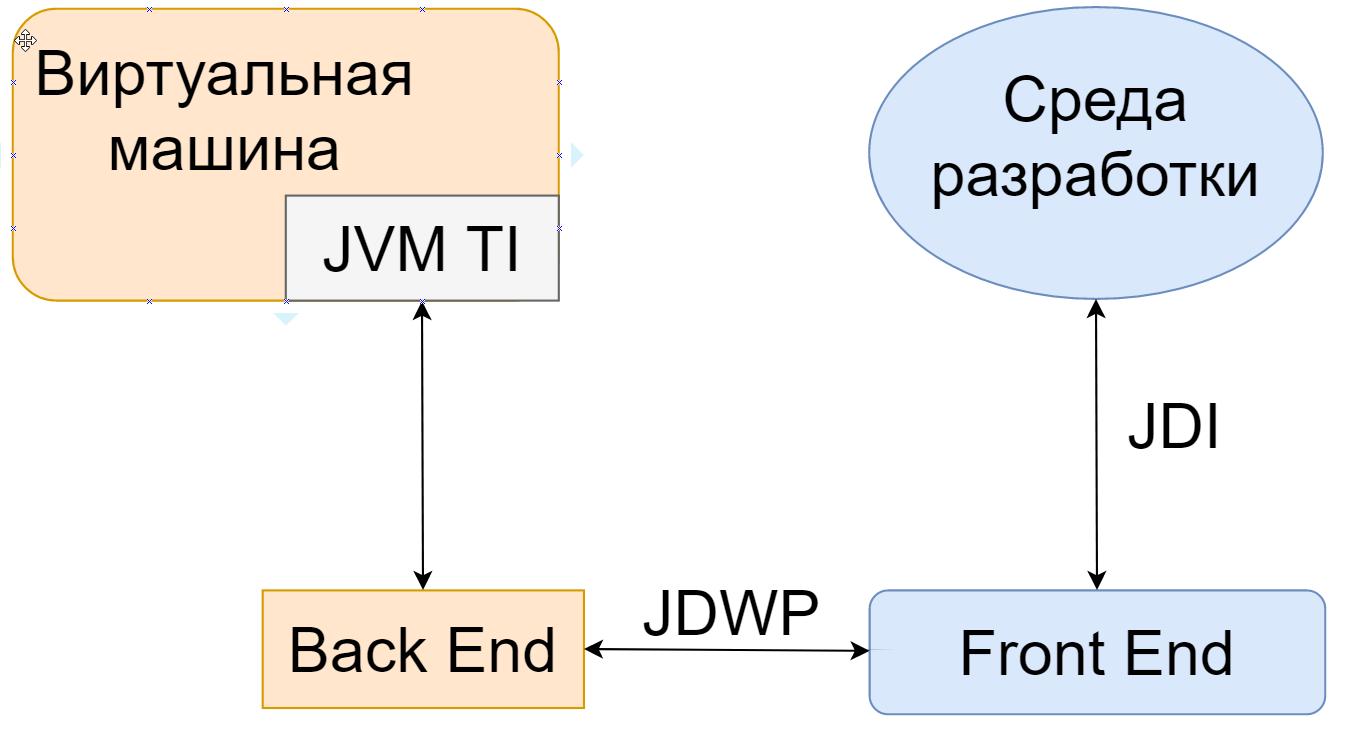
\includegraphics[scale=0.4]{chapter1/img/jdpa.png}

В блоках "Front End" и "Back End" скрыты детали реализации по обмену сообщениями -- очереди сообщений и потоки, обрабатывающие эти сообщения.

JPDA состоит из трех частей:
\begin{itemize}
	\item JVM TI -- Java VM Tool Interface - описывает сервисы, которая предоставляет виртуальная машина для отладки. 
	\item JDWP -- Java Debug Wire Protocol - протокол общения между отладчиком и виртуальной машиной. Описывает формат сообщений между отладчиком и JVM, создавая дополнительную абстракцию и позволяя использовать технологии для написания отладчиков.
	\item JDI -- Java Debug Interface - высокоуровневый Java интерфейс для взаимодействия с виртуальной машиной. Поставляется вместе с JDK, входит в пакет сom.sun.jdi. Содержит набор классов-посредников для сущностей отлаживаемой виртуальной машины (потоки, объекты, классы и т.д.).
\end{itemize}




\subsection{Функции высших порядков} % TODO: назвать нормально
В 2014 году вышла восьмая версия языка программирования Java. Одними из нововведений обновления 
стала поддержка анонимных функций и библиотека функций высшего порядка для обработки 
последовательностей элементов -- пакет java.util.stream. Кроме добавления этого пакета 
изменения коснулись и ранее определённых классов -- для некоторых объектов естественно 
представление в виде последовательности элементов: коллекции и поток ввода.

Поддержка анонимных функций сделало доступным следующий синтаксис.
\inputminted{java}{chapter1/code/Lambda.java}

После этого данную функцию можно вызвать:
\inputminted{java}{chapter1/code/UseLambda.java}

С точки зрения пользователя, такое определение анонимной функции является более короткой версией следующего использования анонимного класса.

\inputminted{java}{chapter1/code/SameAnonymous.java}

Вместе с классами из пакета java.util.stream анонимные функции позволяют создавать следующие конструкции:

\inputminted{java}{chapter1/code/StreamUsage.java}

С точки зрения результата такой вызов эквивалентен следующей последовательности операторов: 

\inputminted{java}{chapter1/code/CyclesUsage.java}

Важно, что последовательность вызовов в цепочке нельзя воспринимать как трансформацию коллекций. Правильно трактовать подобные вызовы именно как поток объектов. Это значит, что из источника берется объект и последовательно проходит через все операции, пока это возможно, затем это повторяется и для всех остальных. Очевидно, что возможны ситуации, когда все элементы их источника не понадобятся. Операции для которых это верно называются \textit{короткозамкнутыми}. Как следствие, допускаются бесконечные источники, то тогда цепочка методов должна содержать хотя бы одну короткозамкнутую операцию, иначе такой вызов никогда не завершится.

Таким образом, пакет java.util.stream предоставляет возможность отказаться от обычных управляющих конструкций в пользу операций в функциональном стиле. Обычно это приводит к краткости кода, скрывая от программиста детали реализации операций, оставляя лишь семантику операций.

\subsubsection{Части вызова Stream API}
Типичное использование классов из java.util.stream состоит из нескольких частей: сначала 
нужно инициализировать поток объектов, затем выполнить над объектами набор преобразований, 
после чего нужно аггрегировать объекты в результирующее значение. Таким образом все операции 
можно разделить на два класса:
\begin{itemize}
	\item \textbf{Промежуточная операция.} Операция, которая возвращает Stream. Преобразует объектов. Это значит, что после вызова таких 
	операций могут измениться объекты внутри потока, или их порядок. Примеры:
	\begin{itemize}
		\item \textit{map} -- заменяет каждый объект новым значением, сохраняя порядок.
		\item \textit{filter} -- оставляет только те объекты, которые удовлетворяют 
		\item \textit{distint} -- оставляет только различные элементы (сравнение по $equals$ \cite{java:equals})
		\item и многие другие (см \cite{java:stream})
	\end{itemize}
	При этом все промежуточные операции можно разбить на две части по возможности хранить состояние:
	\begin{itemize}
		\item Без состояния. Большинство операций, выполняющие локальные действия над одним 
		объектом. Для таких операций гарантируется, что 
		\item С состоянием. Допускается, что такие операции должны считать весь входной 
		поток, прежде чем начнут работу следующие по порядку операции. В стандартной 
		реализации таких операций две - sorted и distinct.
	\end{itemize}
	\item \textbf{Завершающая операция.} Эта операция запускает вычисления и преобразует 
	объекты из потока, которые до неё доходят в некоторый результат. В качестве результата 
	может выступать, произвольный объект. Как правило, это коллекции, массивы, определенные 
	значения из потока (максимум/минимум по какому-то признаку) и другие.
\end{itemize}

Кроме того, можно выделить объект - источник. Он содержит либо способен генерировать поток объектов. В качестве источника могут выступать коллекции, массивы, функция-генератор, каналы вводы.
\inputminted{java}{chapter1/code/IntStream.java}
Массив, переданный параметром методу Arrays.stream является источником
\inputminted{java}{chapter1/code/ZerosStream.java}
Данный вызов создает бесконечный поток нулей. Анонимная функция-генератор является источником.

\subsubsection{Детали реализации Stream API}
В своей реализации потоки объектов в java используют абстракцию Spliterator 
\cite{java:spliterator}, так же введенную в восьмой версии. Spliterator - это интерфейс, 
который усложняет понятие обычного итератора в java -- объекта, который позволяет обойти 
некоторый набор объектов \cite{java:iterator}. Spliterator хранит свойства объектов которые 
обходятся: их количество, упорядоченность, изменяемость, признак того, что данные уже 
отсортированы и другие. Эти свойства могут быть использованы при выполнении операций над 
потоком объектов. Так же в Spliterator добавлен новый метод split, который позволяет 
разделить множество объектов на две непересекающиеся части, и обойти параллельно. На этой идее основывается реализация параллельных потоков параллельных потоков.

Несмотря на то, что java является объектно-ориентированным языком, не все значения в java 
являются объектами. Исключения составляют примитивные типы, для которых хранение в виде 
объектов невыгодно с точки зрения производительности. По этим же причинам, реализация 
java.util.stream содержит отдельную реализацию для объектов примитивных типов -- IntStream, 
LongStream, DoubleStream -- для поддержки потоков целых и вещественных чисел. 

\subsubsection{Расширения стандартной библиотеки}
Стандартная библиотека предоставляет довольно большой набор промежуточных и завершающих операций. Тем не менее существуют расширения базового интерфейса. Примерами таких расширений служат библиотеки - jOOL \cite{java:jool} и StreamEx \cite{java:streamex}.

Они полностью совместимы со стандартной реализацией и дают те же гарантии. Операции, добавленные в этих библиотеках, как правило упрощают написание кода с использованием интерфейса потоков объектов. Хотя многие из новых операций можно выразить через уже имеющиеся.

\subsubsection{Аналоги в других языках}
Идея обрабатывать множества объектов как потоки в императивных языках не новая. В 2007 году Microsoft представил LINQ (язык интегрированных запросов) для языка $C\#$ \cite{ms:linq}. Он предоставляет очень схожие возможности, но дизайн этого расширения отличен от java.util.stream. В реализации были использованы методы-расширения \cite{ms:ext}, а так же ключевое слово yield \cite{ms:yield}. Так же операции названы по аналогии с SQL, тогда как в java операции имеют аналоги в функциональных языках, например Haskell.

Подобные возможности реализуют коллекции в языке Scala \cite{ho:scala} и абстракция Sequence в языке Kotlin \cite{ho:kotlin}.
\subsection{Отладка операций в функциональном стиле}
После появления функций высшего порядка и расширения стандартной библиотеки возможности JPDA остались прежними. Таким образом, с одной стороны, имеется способ записывать операции над множествами объектов в новом синтаксисе, с другой стороны, возможности отладчика остались прежними. Рассмотрим возможности отладчиков трех крупнейших сред разработки (Eclipse, NetBeans, IntelliJ IDEA), которые могут быть полезны при отладке цепочек методов, оперирующих потоком объектов.

\begin{itemize}
	\item Использование точек останова (с условием). Допускается, что точка останова будет внутри тела анонимной функции.
	\item Последовательные переходы по вызовам анонимных функций внутри цепочки.
	\item Вычисление выражений с анонимными функциями (доступно только в IDEA).
\end{itemize}

\subsubsection{Недостатки имеющихся подходов}
% TODO: немного переделать структуру, сейчас как-то неочень
Описанные методы обладают недостатками, их не всегда удобно использовать и не всегда достаточно, чтобы понять причину ошибок.

Перечислим недостатки этих подходов.
\begin{itemize}
	\item При использовании точек останова внутри анонимной функции у нас есть только информация о текущем вызове и объект, при этом нельзя понять почему именно этот объект появился в данном месте, и какие трансформации он претерпел. Логичное предположение, что эту информацию можно восстановить в одном из элементов стека вызовов окажется неверным. Стек вызовов состоит из большого числа внутренних вызовов и нет гарантий, что получится там найти что-то полезное. Ниже приведен пример стека для достаточно простого вызова.
	\inputminted{java}{chapter1/code/SimplestStreamExample.java}
	
	И стек вызовов в точке останова внутри анонимной функции.
	
	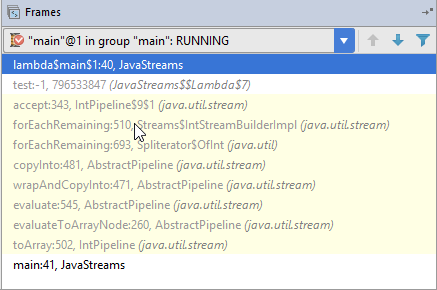
\includegraphics[scale=1.]{chapter1/img/stack.png}
	
	\item Чтобы поставить точку останова, нужно иметь участок кода где нужно остановиться, таким участком кода может выступать, например, вызов анонимной функции. Но не все вызовы предполагают передачу анонимной функции в качестве параметра. Поэтому такой подход применим не для всех цепочек. По этой же причине переходы по последовательным вызовам анонимных функций не всегда возможны.
	
	Пример кода, когда применение точек останова затруднено: \inputminted{java}{chapter1/code/HardToUseBreakpoint.java}
\end{itemize}

Кроме описанных способов можно использовать и другие, но они так же имеют недостатки:
\begin{itemize}
	\item Интерфейс Stream определяет специальный метод peek, который может упростить отладку. Назначение этого метода -- извлечь каждый объект из потока (не изменив логику и последовательность работы потока), и совершить в ним какое-то действие, полезное для отладки. Примером такого действия может быть печать в лог. 
	
	Недостатки: 
	\begin{itemize}
		\item Необходимо модифицировать код.
		\item Не все объекты можно удобно представить в виде строки.
		\item Вычисление потока происходит лениво, поэтому понять получившийся лог будет не так просто.
	\end{itemize}

	\item Некоторые среды разработки позволяют автоматически преобразовать некоторые цепочки методов Stream API в эквивалентный код с циклами. 
	
	Недостатки:
	\begin{itemize}
		\item Не каждая цепочка может быть автоматически преобразована.
		\item Необходимо модифицировать код.
		\item Ошибка может пропасть после трансформации. Так же могут появиться новые.
		\item Обратный переход от циклов к Stream API скорее всего невозможна.
	\end{itemize}
	
	\item Частичное исполнение цепочки с сохранением в промежуточную коллекцию.
	
	Пример: 
	\inputminted{java}{chapter1/code/PartialEvaluationFull.java}
	
	Дополнительно можно вычислить два выражения:
	\inputminted{java}{chapter1/code/PartialEvaluation1.java}
	
	\inputminted{java}{chapter1/code/PartialEvaluation2.java}
	
	В результате у нас есть данные о промежуточных состоянии.
	
	Недостатки:
	\begin{itemize}
		\item Не все вызовы Stream API допускают частичное исполнение. Бесконечные потоки с короткозамкнутыми операциями аналогично сделать не позволят, придется добавлять дополнительные операции, такие как limit.
		\item Не позволяет отследить историю трансформаций объекта.
		\item Доступно не во всех средах разработки и не для всех анонимных функций.
	\end{itemize}
\end{itemize}

Таким образом, нет удобного способа, который бы позволил увидеть как трансформируются объекты внутри потока.

\subsubsection{Решение для C\#. OzCode}
В языке C\# имеются аналогичные проблемы. Но существует расширение среды разработки Visual Studio, которое упрощает отладку цепочек LINQ методов. Этот проект называется OzCode. Это платное расширение Visual Studio с закрытым исходным кодом. В конце 2016 года в нём появилась новая функция - отладчик LINQ. 






\subsection{Постановка задачи}
Цель данной работы -- расширить возможности встроенного в среду разработки IntelliJ IDEA отладчика для упрощения отладки операций в функциональном стиле.

Для того, чтобы выполнить эту цель, поставим следующие задачи
\begin{itemize}
	\item Определить вызовы с использованием операций в функциональном стиле среди доступных из текущей позиции отладчика;
	\item Получить информацию о трансформациях каждого объекта в потоке объектов;
	\item Визуализировать результаты.
\end{itemize}


%\begin{frame}
\frametitle{Overview} % Table of contents slide, comment this block out to remove it
\tableofcontents % Throughout your presentation, if you choose to use \section{} and \subsection{} commands, these will automatically be printed on this slide as an overview of your presentation
\end{frame}

%----------------------------------------------------------------------------------------
%   PRESENTATION SLIDES
%----------------------------------------------------------------------------------------

%------------------------------------------------
\section{First Section} % Sections can be created in order to organize your presentation into discrete blocks, all sections and subsections are automatically printed in the table of contents as an overview of the talk
%------------------------------------------------

\subsection{Subsection Example} % A subsection can be created just before a set of slides with a common theme to further break down your presentation into chunks

\begin{frame}
\frametitle{Paragraphs of Text}
Sed iaculis dapibus gravida. Morbi sed tortor erat, nec interdum arcu. Sed id lorem lectus. Quisque viverra augue id sem ornare non aliquam nibh tristique. Aenean in ligula nisl. Nulla sed tellus ipsum. Donec vestibulum ligula non lorem vulputate fermentum accumsan neque mollis.\\~\\

Sed diam enim, sagittis nec condimentum sit amet, ullamcorper sit amet libero. Aliquam vel dui orci, a porta odio. Nullam id suscipit ipsum. Aenean lobortis commodo sem, ut commodo leo gravida vitae. Pellentesque vehicula ante iaculis arcu pretium rutrum eget sit amet purus. Integer ornare nulla quis neque ultrices lobortis. Vestibulum ultrices tincidunt libero, quis commodo erat ullamcorper id.
\end{frame}

%------------------------------------------------

\begin{frame}
\frametitle{Bullet Points}
\begin{itemize}
\item Lorem ipsum dolor sit amet, consectetur adipiscing elit
\item Aliquam blandit faucibus nisi, sit amet dapibus enim tempus eu
\item Nulla commodo, erat quis gravida posuere, elit lacus lobortis est, quis porttitor odio mauris at libero
\item Nam cursus est eget velit posuere pellentesque
\item Vestibulum faucibus velit a augue condimentum quis convallis nulla gravida
\end{itemize}
\end{frame}

%------------------------------------------------

\begin{frame}
\frametitle{Blocks of Highlighted Text}
\begin{block}{Block 1}
Lorem ipsum dolor sit amet, consectetur adipiscing elit. Integer lectus nisl, ultricies in feugiat rutrum, porttitor sit amet augue. Aliquam ut tortor mauris. Sed volutpat ante purus, quis accumsan dolor.
\end{block}

\begin{block}{Block 2}
Pellentesque sed tellus purus. Class aptent taciti sociosqu ad litora torquent per conubia nostra, per inceptos himenaeos. Vestibulum quis magna at risus dictum tempor eu vitae velit.
\end{block}

\begin{block}{Block 3}
Suspendisse tincidunt sagittis gravida. Curabitur condimentum, enim sed venenatis rutrum, ipsum neque consectetur orci, sed blandit justo nisi ac lacus.
\end{block}
\end{frame}

%------------------------------------------------

\begin{frame}
\frametitle{Multiple Columns}
\begin{columns}[c] % The "c" option specifies centered vertical alignment while the "t" option is used for top vertical alignment

\column{.45\textwidth} % Left column and width
\textbf{Heading}
\begin{enumerate}
\item Statement
\item Explanation
\item Example
\end{enumerate}

\column{.5\textwidth} % Right column and width
Lorem ipsum dolor sit amet, consectetur adipiscing elit. Integer lectus nisl, ultricies in feugiat rutrum, porttitor sit amet augue. Aliquam ut tortor mauris. Sed volutpat ante purus, quis accumsan dolor.

\end{columns}
\end{frame}

%------------------------------------------------
\section{Second Section}
%------------------------------------------------

\begin{frame}
\frametitle{Table}
\begin{table}
\begin{tabular}{l l l}
\toprule
\textbf{Treatments} & \textbf{Response 1} & \textbf{Response 2}\\
\midrule
Treatment 1 & 0.0003262 & 0.562 \\
Treatment 2 & 0.0015681 & 0.910 \\
Treatment 3 & 0.0009271 & 0.296 \\
\bottomrule
\end{tabular}
\caption{Table caption}
\end{table}
\end{frame}

%------------------------------------------------

\begin{frame}
\frametitle{Theorem}
\begin{theorem}[Mass--energy equivalence]
$E = mc^2$
\end{theorem}
\end{frame}

%------------------------------------------------

\begin{frame}[fragile] % Need to use the fragile option when verbatim is used in the slide
\frametitle{Verbatim}
\begin{example}[Theorem Slide Code]
\begin{verbatim}
\begin{frame}
\frametitle{Theorem}
\begin{theorem}[Mass--energy equivalence]
$E = mc^2$
\end{theorem}
\end{frame}\end{verbatim}
\end{example}
\end{frame}

%------------------------------------------------

\begin{frame}
\frametitle{Figure}
Uncomment the code on this slide to include your own image from the same directory as the template .TeX file.
%\begin{figure}
%\includegraphics[width=0.8\linewidth]{test}
%\end{figure}
\end{frame}

%------------------------------------------------

\begin{frame}[fragile] % Need to use the fragile option when verbatim is used in the slide
\frametitle{Citation}
An example of the \verb|\cite| command to cite within the presentation:\\~

This statement requires citation \cite{p1}.
\end{frame}

%------------------------------------------------

\begin{frame}
\frametitle{References}
\footnotesize{
\begin{thebibliography}{99} % Beamer does not support BibTeX so references must be inserted manually as below
\bibitem[Smith, 2012]{p1} John Smith (2012)
\newblock Title of the publication
\newblock \emph{Journal Name} 12(3), 45 -- 678.
\end{thebibliography}
}
\end{frame}

%------------------------------------------------

\begin{frame}
\Huge{\centerline{The End}}
\end{frame}

%----------------------------------------------------------------------------------------

\end{document}